\PassOptionsToPackage{unicode=true}{hyperref} % options for packages loaded elsewhere
\PassOptionsToPackage{hyphens}{url}

\documentclass[11pt]{article}

% Any additional packages needed should be included after obs_study_style.
% Note that obs_study_style.sty includes epsfig, amssymb, natbib and graphicx,
% and defines many common macros, such as 'proof' and 'example'.
%
% It also sets the bibliographystyle to plainnat; for more information on
% natbib citation styles, see the natbib documentation, a copy of which

%\usepackage{obs_study_style}

% Definitions of handy macros can go here

\usepackage[small]{caption} %small font captions
%\usepackage{parskip} %for no indent and more space in between paragraphs
\usepackage[letterpaper,bottom=1in,top=1in,right=1.25in,left=1.25in,includemp=FALSE,includeheadfoot=FALSE,headheight=0pt]{geometry}
\usepackage{ctable}
\usepackage[natbib=true,backend=biber,style=chicago-authordate]{biblatex}
\addbibresource{refs.bib}
\usepackage{float}
\usepackage{enumitem}
\usepackage{comment}
\usepackage{lmodern}
\usepackage[utf8]{inputenc}
\usepackage{amssymb,amsmath}
\usepackage{ifxetex,ifluatex}
\usepackage{multirow}
\usepackage{multicol}
\usepackage[colorlinks  = true,
            linkcolor   = blue,
            urlcolor    = blue,
            citecolor   = blue,
            anchorcolor = white]{hyperref}
%\usepackage{fixltx2e} % provides \textsubscript
\ifnum 0\ifxetex 1\fi\ifluatex 1\fi=0 % if pdftex
  \usepackage[T1]{fontenc}
  \usepackage[utf8]{inputenc}
  \usepackage{textcomp} % provides euro and other symbols
\else % if luatex or xelatex
  \usepackage{unicode-math}
  \defaultfontfeatures{Ligatures=TeX,Scale=MatchLowercase}
\fi
% use upquote if available, for straight quotes in verbatim environments
\IfFileExists{upquote.sty}{\usepackage{upquote}}{}
% use microtype if available
\IfFileExists{microtype.sty}{%
\usepackage[]{microtype}
\UseMicrotypeSet[protrusion]{basicmath} % disable protrusion for tt fonts
}{}
\IfFileExists{parskip.sty}{%
\usepackage{parskip}
}{% else
\setlength{\parindent}{0pt}

\setlength{\parskip}{6pt plus 2pt minus 1pt}
}

\usepackage{xcolor}
\usepackage{soul}

\usepackage{hyperref}
\hypersetup{
            pdfborder={0 0 0},
            breaklinks=true}
\urlstyle{same}  % don't use monospace font for urls
\usepackage{longtable,booktabs}
\usepackage{pdflscape}
\usepackage{lscape}
\usepackage{rotating}
% Fix footnotes in tables (requires footnote package)
\IfFileExists{footnote.sty}{\usepackage{footnote}\makesavenoteenv{longtable}}{}
\usepackage{graphicx,grffile}
\makeatletter
\def\maxwidth{\ifdim\Gin@nat@width>\linewidth\linewidth\else\Gin@nat@width\fi}
\def\maxheight{\ifdim\Gin@nat@height>\textheight\textheight\else\Gin@nat@height\fi}
\makeatother
% Scale images if necessary, so that they will not overflow the page
% margins by default, and it is still possible to overwrite the defaults
% using explicit options in \includegraphics[width, height, ...]{}
\setkeys{Gin}{width=\maxwidth,height=\maxheight,keepaspectratio}
\setlength{\emergencystretch}{3em}  % prevent overfull lines
\providecommand{\tightlist}{%
  \setlength{\itemsep}{0pt}\setlength{\parskip}{0pt}}
% \setcounter{secnumdepth}{0}
% Redefines (sub)paragraphs to behave more like sections
\ifx\paragraph\undefined\else
\let\oldparagraph\paragraph
\renewcommand{\paragraph}[1]{\oldparagraph{#1}\mbox{}}
\fi
\ifx\subparagraph\undefined\else
\let\oldsubparagraph\subparagraph
\renewcommand{\subparagraph}[1]{\oldsubparagraph{#1}\mbox{}}
\fi

% set default figure placement to htbp
\makeatletter
\def\fps@figure{htbp}
\makeatother


\newcommand{\dataset}{{\cal D}}
\newcommand{\fracpartial}[2]{\frac{\partial #1}{\partial  #2}}

% For papers submitted for review, just fill in author names
% For accepted papers, heading arguments are {volume}{year}{pages}{submitted}{published}{author-full-names}
%\heading{}{Repetto}{}

% Short headings should be running head and authors last names


\author{Rosario Queirolo\thanks{Universidad Católica del Uruguay (\url{rosario.queirolo@ucu.edu.uy})}
	\and Jake Bowers\thanks{University of Illinois @ Urbana-Champaign}
	\and Eliana Álvarez\thanks{Universidad Católica del Uruguay}
	\and Lorena Repetto\thanks{Universidad Católica del Uruguay}}

\title {The Impact of Marijuana Sale at Pharmacies on Crime Victimization and Insecurity Perceptions.\thanks{This research was supported by Open Society Foundations funds OR2017-35193 and OR2016-27307, and the National Agency for Research and Innovation (ANII) between 2017 and 2019.}}

\graphicspath{{.}{Analysis/}{media/}{figs/}}

\begin{document}
%\firstpageno{1}

\maketitle

 
\begin{abstract}

Do drugs' legalization have an impact on crime and public security? This paper presents the results of an observational design that evaluates the impact that recreational marijuana sale at pharmacies had on insecurity perceptions and crime victimization in Uruguay. Evidence about the impact of legal marijuana dispensaries on crime is mixed. Furthermore, Uruguay´s crime rates are consistently increasing in the last five years, which is an important difference with main evidence coming from studies carried out in the United States, where national crime rates have the opposite trend. Less is known about how this kind of policies affect people´s perceived public insecurity. We performed two surveys, one before and one after the implementation of the selling at pharmacies started. The sample is composed by 1.298 neighbors of 64 pharmacies in all the territory, 10 or more neighbors per pharmacy in each round. These outcomes included country’s insecurity perception, neighborhood’s insecurity perception, crime victimization in the last twelve months, perceived impact on public insecurity, perceived impact on drug trafficking, reported existence of ``bocas'', insertion in the neighborhood and social disorder. Data is analyzed by differences in differences (DD) to estimate the causal effect before and after the implementation of the marijuana regulation. We found no significant impact of closeness to dispensaries on crime victimization. Neither on public insecurity. This result add to part of the research done on the impact of marijuana legalization in several US states. We do find an impact on the perception of drug trafficking: neighbors of marijuana selling pharmacies consider that the legalization had a positive impact on traffic. While we cannot pin down the mechanisms behind this effect, we believe that seeing users buying legal marijuana might lead citizens to think that illegal deals have diminished.
\end{abstract}
%\begin{keywords}
% Crime, Legal Marijuana dispensaries, Natural experiment, insecurity perception
%\end{keywords}

\section[]{Laws, Norms, and the Sale of Marijuana in Neighborhoods in Uruguay}

In 2013, Uruguay became the first country in the world to fully regulate the production, distribution and commercialization of marijuana. The December 2013 law fully implemented in 2017 had three main objectives via  regulation of marijuana:  users' decriminalization, reduce public insecurity and drug-trafficking related violence, and increase public health through education and risk reduction and prevention campaigns now made easy to implement because of their reference to a legal substance \citep{arraras2014inventando, pardo2014cannabis, queirolo2019uruguay}. Although access to marijuana was regulated via cannabis club memberships and self-cultivation before July 2017, on July 19, 2017 the public was first allowed to buy marijuana at licensed pharmacies. Much of the Uruguayan public opposed the legalization of in general and the normalization of marijuana usage via the sale of marijuana at pharmacies in particular: only 16 out of more than 1000 pharmacies registered to sell marijuana by the July 2017 date. This paper focuses on pharmacies because the sale of marijuana by a pharmacy has the potential to bring non-marijuana users in the neighborhood into daily and ordinary contact with people buying and using marijuana in public. The other changes created by the law tended to either improve the private use of marijuana by people already using it or created some legal conditions for farmers newly cultivating the plant or those previously distributing marijuana illegally. Thus, a pharmacy-level change is, in the context of pharmacies and neighborhoods in Uruguay, a neighborhood level change: would daily contact with a marijuana selling pharmacy and its users have an impact on public insecurity perceptions and crime victimization? To learn about the dynamics of this process and to document them, our research team fielded in-person interviews of roughly 10 neighbors of each of the 16 registered pharmacies as well as with 10 neighbors living near 42 pharmacies chosen to be similar to the 16 registered pharmacies but which had not registered to sell marijuana during the month before sale of marijuana was made legal. We also re-surveyed those neighborhoods (and some  of the same neighbors in a small panel) one year later, in August of 2018.

\paragraph{Why document the effect of the sale of marijuana on attitudes?}\\
A government aiming to achieve positive policy objectives like less violence and better health opposed by a public with negative stereotypes and norms is not unique to the Uruguayan case. The desegregation of schools in the USA, the legalization of same-sex marriage in the USA and elsewhere, the legalization of divorce and abortion in predominantly Catholic countries, laws against underage marriage in Muslim countries, and laws facilitating women participation in public office in India, are all examples of law running ahead of norms. The law changes before norms, in part, because elites aim to use law and regulation to change norms themselves \citep{beaman2009powerful,Tankard:2016, Tankard:2017}. In Uruguay, for example, one of the mechanisms by which the legal change would produce positive effects is if marijuana users no longer need to hide their behavior for  fear of social sanction.

We hope to contribute to the public policy discussion in Uruguay and elsewhere on whether, on balance, legalization of marijuana has produced social goods or not. In particular, this paper analyze the impact of marijuana legalization in one of the law objectives: reduce public insecurity and crimes.Research has found mixed results about the relationship between legalization and crime in general. For example, \cite{braakmann2014cannabis} and \cite{chu2019joint} at national level find no significant relationship between medical marijuana laws and crime. In Denver, Colorado, two articles find contradictory evidence: while \citep {freisthler2016micro} show that the impact of availability of marijuana dispensaries on crime does not occur where the outlets are located, and it might occur in adjacent areas; \citep {brinkman2019not} finds that an additional dispensary has a significant impact on reducing on crime on the neighborhood with no spillover effects to adjacent areas. Evidence from experimental or quasi-experimental research has shown a decrease in some types of crimes \citep{dragone2019crime, gavrilova2014legal, hao2017cross, Indigo:2016} --- in the context of a  sustained downward trend in national crime rates in the USA \citep{gramlich5facts}. In Uruguay, the situation is the opposite: national crime trends show a significant increase in last years \citep{paternain2008panorama}, so we should not expect that legalization would have the same effect than in contexts where crime has been diminishing \citep {eisner2016achieving}.

There is less evidence about the direct impact of legalization on insecurity perceptions, although we imagine that changes in actual crime rates and victimization might matter for perceptions. We know that simple perceptions of demographics of neighborhoods often diverge from census reported figures (\citep{wong2012bringing}, and we also know that fear of crime does not necessarily reflect the prevalence of crime or the probability of crime (\citep{wong2012bringing}. This fact, that the picture of crime in the head of a person may not be the picture shared by a local police department or criminologist, means that we do not have strong priors about how a pharmacy may change such perceptions by our survey sample: if perceptions are malleable, then perhaps a new pharmacy might lead to quick change; if, on the other hand, people ignore their surroundings and/or only perceive that which fits in which their previous beliefs, then perhaps the pharmacies may have no effects.

The rest of the paper is structured as follow. Section two describes the context, in particularly, the way in which the public security argument was introduced in the implementation of marijuana selling at pharmacies and how the selling currently works. The third section summarizes the evidence about the relationship between marijuana legalization and crime, describes the main outcomes we are looking at,  and states our main hypotheses. Fourth, we explain our research design. In the fifth section, results are presented; and in the sixth section we discuss how well or bad our design deals with unobserved confounds. Finally, we end up with a discussion section.

\section{Marijuana retail at pharmacies: a controversial measure}

From over 1000 pharmacies operating in Uruguay, only 16 decided to start selling marijuana on July 19, 2017. The reasons given by some pharmacists for not entering the system varied. Some of them rejected the idea of selling a recreational drug; other pharmacy owners claimed uncertainty about the functioning of the system. Still others worried about the economic profitability of the initiative or about the potential threat to their security and reprisals from dealers \citep{boidi2016}. Currently, the Institute of Regulation and Control of Cannabis (IRCCA) reports 17 pharmacies active in the dispensary system, located in only 10 of the 19 departments of the country.

Main opposition to the idea of selling marijuana at pharmacies came from associations of the pharmaceutical industry. Even before its implementation, the main professional organizations of pharmacists and owners of pharmacies came out against the measure.\footnote{These organizations included the professional organization of pharmaceutical chemists (the Association of Chemistry and Pharmacy of Uruguay (AFQU)), and the professional organization of owners of pharmacies in Montevideo (the Pharmaceutical Chamber (CF)) and the Association of Pharmacies of the Interior (AFI).} For example, the Association of Chemistry and Pharmacy of Uruguay publicly stated that pharmacies exist to provide healthcare and the sale of a recreational drug was not consistent with the primary purpose of pharmacies. The Association of Pharmacies of the Interior voiced concerns about public security: ``There is a lot of fear of becoming highly attractive for thieves, especially on peripheral pharmacists''\footnote{Diario El Pais.``Marijuana: pharmacies fear assaults''. Published on May 9, 2016. In: \url{https://www.elpais.com.uy/informacion/marihuana-farmacias-temen-asaltos.html} Original quote in spanish: ``Hay mucho temor de que sean posibles llamadores de asaltos, especialmente farmacias periférica''}. In the same newspaper article, the professional organization of owners of pharmacies in Montevideo expressed the same concerns: ``We all know that pharmacies are highly precious for criminals. Pharmacists had been killed, and in poor neighborhoods on the edges of the city, people steal to buy a joint and now marijuana will be in the pharmacies''\footnote{Diario El Pais. "Marijuana: pharmacies fear assaults". Published on May 9, 2016. In: \url{https://www.elpais.com.uy/informacion/marihuana-farmacias-temen-asaltos.html} Original quote in Spanish:"Todos sabemos que la farmacia barrial es un botín muy preciado para los delincuentes. Hemos tenido farmacéuticos asesinados y en barrios periféricos te roban para comprar un porro y ahora la marihuana va a estar en la propia farmacia"}.

Security concerns were also present at the time of the implementation of marijuana legalization in the United States, where the legalization wave produced concerns about the crime impact of this kind of permissive drug policy. For instance, in October 2016, the Denver District Attorney wrote a letter warning Californian citizens that have voted for Proposition 64 (Adult Use of Marijuana Act) about the effect of recreational marijuana legalization on the raising of crime in Denver and Colorado \citep{dragone2019crime}.

Out of the three mechanisms of legal access to marijuana in Uruguay, the sale in pharmacies is the only one that forces contact between users and non-users. This visibility does not happen with the cannabis clubs nor with domestic cultivation. Moreover, the sale of marijuana in stores that also trade other non-related products, such as pharmacies, represents an innovation in comparison with other marijuana legalization experiences such as the Colorado and Washington initiatives, where cannabis is sold in specialized stores. In this sense, the Uruguay regulation forced contact between those supporting the law, and personally benefiting from it, and those opposing it. And this contact, in turn, motivates our research design.

\section{Outcomes: Crime, Insecurity Perceptions and Perceived Impacts of Marijuana Legalization}

Why might sale of marijuana in local pharmacies change crime victimization, fear of crime and insecurity perceptions? One possible avenue is that legalization of marijuana might increase marijuana use, and increased marijuana might increase crime (which would in turn be perceived or directly experienced by neighbors leading to a higher public perception of insecurity). Other related way is that pharmacies became more attractive for thieves because they sell marijuana. This is the argument that many pharmacies owners claimed for not adhering to the selling.

On the contrary, the hopes motivating the passage of Law 19.172 (the law legalizing marijuana in Uruguay) were reducing drug related crimes by removing marijuana users from the illegal market and undermining the economic power of drug trafficking. Following the government's goal, we could expect that the sale of marijuana in pharmacies will reduce crime and increase public security because dealers and illegal selling points ``bocas'' will move away from the neighborhood.

Evidence on the causal relationship among drugs and perception of public insecurity and actual victimization is mixed. While some scholars show strong evidence supporting the link between illicit drug use and crime \citep{white2000dynamics}, others point to the complexity of the relationship, as well as the spurious and/or recursive nature of observed relationships. \citep{gottfredson1990general, mcbride1993drugs}.\footnote{For a review of this literature, see \citet{brothers2003substance}.} In Latin America, evidence of this causal relationship is even weaker because most of the research is based on criminal samples that biased results towards a significant effect \citet{trajtenberg2018self}.

Drugs may cause crime, in theory, either because of ‘psychopharmacological violence’ (crime occurs as a consequence of drug consumption), but also by ‘economic compulsive violence’ (crime as a result of certain individuals’ actions involved in illegal economic practices to cost their personal consumption) and or ‘systemic violence’ (crime becomes related to drug trafficking and distribution) \citep{goldstein1985drugs}.

Cannabis use occupies a particular place in the drug/violence nexus discussion because most studies have concluded that marijuana consumption tends to inhibit violent behavior in the short term, disqualifying the psychopharmacological argument \citep{white2000dynamics}.\footnote{Although a review by the National Research Council concluded that long-term cannabis use can affect the nervous system prompting violence behavior \citep{national1994understanding}.} By the same reasoning, marijuana use rarely generates economic violence as it does not produce the compulsive need to generate income to fund consumption since marijuana is relatively cheap \citep{caulkins2016marijuana}. Finally, given the low profitability of marijuana markets in comparison with other drugs, such as cocaine and heroin, observers believe that marijuana use does not play a significant part in the systemic type of violence \citep{pacula2003marijuana, caulkins2015considering}. Thus, the legalization of marijuana should not have large short term effects on violence unless the removal of marijuana from the portfolios of illegal dealers somehow increases violence and competition in the cocaine and other drug markets.

Despite these reasons, recent evidence for the US states that have legalized marijuana shows that these laws have an effect on the reduction of violent crimes and property crimes \citep{dragone2019crime, Indigo:2016, gavrilova2014legal, huber2016cannabis,brinkman2019not, hao2017cross}. The causal mechanisms behind these relationships are still unclear. They might be: 1) that the psychotropic effect of consuming marijuana is sedative, which decreases the chances of getting involved in violent crimes \citep{no2001health, green2003being}; or 2) that users of alcohol and other drugs are substituting their consumption with marijuana which is a less violent drug \citep{anderson2014legalization, kelly2014policing} ; or 3) that the decrease in crime rate is an effect of the reallocation of police efforts which after the legalization does not need to prosecute marijuana consumption \citep{adda2014crime}; or 4) that by withdrawing the sale of marijuana from unsafe places and placing it in legal and secure contexts, criminal gangs, intermediaries and dealers become weaker \citep{becker2013have}. This evidence comes from the USA where trends in crime show a drop in time \citep{gramlich5facts, james2018recent}. This is not the case in Uruguay, where reports of homicides, robberies and assaults rates have been increasing at least since 2012, as we can see on Figure~\ref{fig:homrap19802017}.

\begin{figure}[H]
\begin{center}
    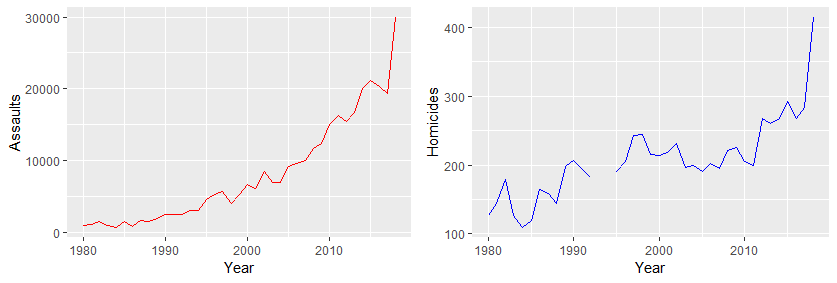
\includegraphics{evo_delitos.png}
    \caption{Number of homicides and assaults in Uruguay. 1980 - 2018.  Source: Observatorio de Violencia y Criminalidad del Ministerio del Interior.}
    \label{fig:homrap19802017}
\end{center}
\end{figure}

Not only crime has been increasing in Uruguay, also public concern towards insecurity. Public opinion studies show that public insecurity is one of the most important problems for Uruguayans: 61\% of Uruguayans considered "Insecurity" as the main problem of the country, even though 51\% of them never experienced a crime \footnote{CIFRA (July 2018) http://www.cifra.com.uy/index.php/2018/08/20/inseguridad-el-problema-mas-grave-que-afecta-mas-a-jovenes-y-mujeres/}. This proportion has been increasing since 2007, even before the crime rate peaked.

It has been well established that personal crime experiences -victimization- are one of the most important predictors of insecurity perceptions \citep{cruz2009public}. This means that people who were victimized by crime tend to feel more insecure than those who did not, even if they live in the same area. But, as we mentioned, fear of crime does not necessarily correspond to actual crime rates and their trends \citep{wong2012bringing}; other elements influence peoples' perceptions regarding public safety and the possibility of experience a crime. Neighborhood´s social daily dynamics, infrastructure and general environment, also play a role in insecurity perceptions. Social conditions of neighborhoods can influence how people feels in terms of safety \citep{cruz2009public, brunton2011neighborhoods, valera2014perceived}. Studies have named these conditions as \textit{social disorder} or \textit{incivilities}. Situations like loitering, people drinking on the streets, gangs' presence, street harassment, etc. \citep{bennett1994determinants, valera2014perceived} are usually used to illustrate signs of social disorder. As more common or frequent these situations become, more unsafe people feel, generating a direct relation between social disorder and fear of crime.

People using and/or buying drugs in public spaces can also be considered a sign of social disorder. Social stereotype of drug users usually conceived them as unpredictable, and therefore, a threat to their neighbors \citep{bennett1994determinants}. Social contact produced by sale at pharmacies between marijuana users and non-users neighbors, either at the  moment of the purchase or because of the long lines at the pharmacies' entrance \footnote{Agencia EFE. "Uruguayans make long lines to buy marijuana at pharmacies". Published on July 19, 2017. In: \url{https://www.efe.com/efe/america/sociedad/uruguayos-hacen-largas-colas-para-comprar-marihuana-en-las-farmacias/20000013-3330652} Original quote in spanish:"Uruguayos hacen largas colas para comprar marihuana en las farmacias"}, might be having an effect on the perceived social disorder of the neighborhood where the selling pharmacy is located, and by this, influencing neighbors' fear of crime.

Do we expect that neighborhood pharmacies selling marijuana should change local direct experience with crime and/or public perceptions of safety? We interpret the research based in the US states as arguing against increasing criminal victimization and pointing out a diminishing effect. Yet crime is rising in Uruguay, and concerns about safety have been increasing in Uruguay as well, even before crime began to rise. So, we will take some care to ensure that our comparisons of survey respondents and neighborhoods below do not confuse differences in public security perceptions caused by overall trends with differences that we can attribute to the introduction of marijuana sales at local pharmacies.

\subsection{Outcome Variables}
The main outcomes that we are looking at are crime and insecurity perceptions. We measure crime by asking neighbors if they have experienced a crime in the last 12 months. In order to measure public insecurity perceptions, we use two variables: public insecurity perception in the neighborhood and public insecurity perception in the country. Among these two variables, we expect that marijuana selling pharmacies would have a higher effect on how secure or insecure citizens feel in the neighborhood rather than in the country.

To better understand the impact on public insecurity perceptions, we include three other outcome variables that we argue are related with public insecurity perceptions and fear of crime. First, we use an index that measure social disorder in the neighborhood composed by three variables: presence of young people loitering, presence of drunk or stoned people in the streets, and presence of people arguing with each other. This information was registered by the interviewer looking at the street where the respondent lives, after the face to face interviews were finished. Second, we include a variable that measures if neighbors know about the existence of illegal selling points (``bocas'') in the neighborhood. Considering that ``bocas'' bring illegal activities to the neighborhood which might imply violence, knowing that there is a ``boca'' close by  would be related with citizens insecurity perceptions. Third, we build an index that measure citizens insertion in the neighborhood comprised by four dimensions: use of services (education and health) in the neighborhood, contact among neighbors (chat and/or meet for collective action activities), perform recreational activities in the neighborhood, and shopping in the neighborhood. Neighborhood insertion might be also related to public insecurity perception and fear of crime.

Finally, we considered two outcomes concerning the perceived impacts of the legalization on public safety and drug-trafficking, which are among the main goals of the law. Having a marijuana selling pharmacy in the neighborhood might have an effect on how citizens evaluate the results of the legalization. Neighbors might see marijuana users buying at a pharmacy and conclude that legalization is hindering the illegal market. More details on how these variables are measured and indexes constructed are in Appendix B.

\subsection{Primary Hypotheses}
We list the primary hypotheses of the study below.

\begin{itemize}
\item [\textbf{H1}] \textit{The sale of marijuana at pharmacies will not have significant effects on crime victimization of pharmacies' neighbors}

\item [\textbf{H2}] \textit{The sale of marijuana at pharmacies will not have significant effects on neighbors' insecurity perceptions}

\item [\textbf{H3}] \textit{The sale of marijuana at pharmacies will push ``bocas'' outside the neighborhood}

\item [\textbf{H4}] \textit{The sale of marijuana at pharmacies will increase social disorder in the neighborhood}

\item [\textbf{H5}] \textit{The sale of marijuana at pharmacies will diminish citizens' insertion in the neighborhood}

\item [\textbf{H6}] \textit{The sale of marijuana at pharmacies will not change citizens' evaluations about the impact of marijuana legalization on public security}

\item [\textbf{H7}] \textit{The sale of marijuana at pharmacies will improve citizens' evaluations about the impact of marijuana legalization on drug trafficking}

\end{itemize}

\section{Research Design: Comparing pharmacies and neighbors' attitudes}

The implementation of the selling of marijuana at pharmacies occurred in stages. As a result of this, we were able to build a baseline in June 2017 prior to the beginning of the selling by surveying neighbors that live close to marijuana selling pharmacies and neighbors of non-selling pharmacies, and  a year after the implementation started, during August 2018, we applied the same measurements in a second round of the survey. We also interviewed one representative of each pharmacy in both rounds. In total, we conducted 119 surveys with representatives (59 in 2017 and 60 en 2018). Because marijuana selling was not randomly assigned by the government to pharmacies, and each pharmacy decided to adhere or not to the selling, those that sell and those that do not sell might be different. The data from the pharmacies' representatives survey  allowed us to characterize selling and non-selling pharmacies, and analyze if there were any initial differences between them that could explain the differences on outcomes. 

In terms of infrastructure both selling and non-selling pharmacies are quite similar:  described in most cases as "family business", with an average of five employees, and around 40 years established in the neighborhood. They are also similar regarding security measures, insecurity perceptions and crime victimization, which goes against the idea that pharmacies that sell marijuana did so because they are better equipped in terms of security protection and placed in safer neighborhoods. Despite the rate of non-selling pharmacies that were victims of a crime in the last 12 months is somewhat higher than the rate of selling pharmacies, more representatives of selling pharmacies reported the existence of illegal drugs selling points in the pharmacy' area. 

The important distinction among sellers and non-sellers is concerning opinions towards the public policy, the substance and its users. Owners and representatives of pharmacies that decided to sell are consistently more in favor of the regulation and anticipate it would have more positive impacts, and have less negative opinions towards marijuana users and the substance than non-sellers (see Table \ref{tab:pharmaciesperceptions} in Appendix A). 

\subsection{Baseline and Outcome Data Collection: The Pharmacy Neighbors Survey}

The baseline survey was collected during June 2017, one month before pharmacies were allowed to sell marijuana. At that time the list of pharmacies that were going to sell was not public, as a result, neighbors did not know if the pharmacy close by was going to be a marijuana selling pharmacy. Our field team visited and surveyed 10 neighbors in each of the 60 pharmacies: 16 which had registered to sell marijuana, 42 that had not registered to sell marijuana, and 2 pharmacies that initially were willing to join the sale but never actually did it (placebos). Figure 3 shows the geographical distribution of the pharmacies in our study.

\begin{figure}[htpb!]
    \centering
     \label{fig:ctrltrtpharms_1}
    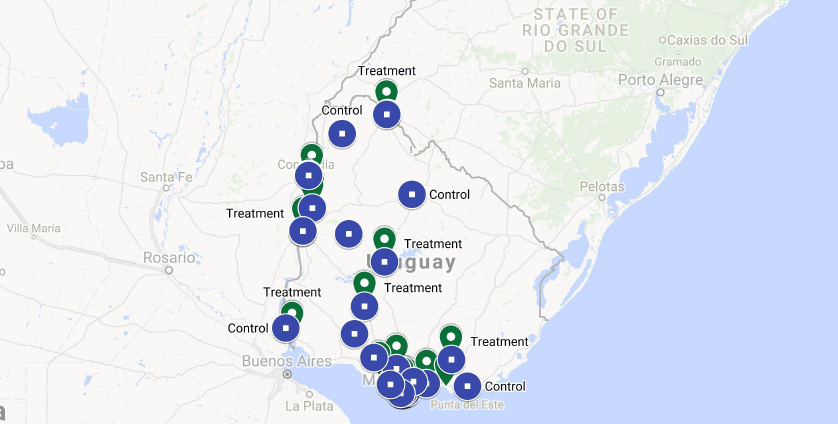
\includegraphics[width=6in,height=5.6851in]{./media/country.png}
    \caption{Pharmacies registered to sell marijuana and comparison pharmacies. Green symbols show pharmacies registered to sell marijuana as of June 2017. Blue symbols are comparison pharmacies.}
\end{figure}

To create a pool from which to sample the 42 pharmacies for the non-selling comparison group we applied four criteria. The first criteria was``same  geographical unit'':  pharmacies in ``departamento'' without at least one selling pharmacy were deleted from the sampling frame. The second criteria was ``population density'':  pharmacies in rural areas were deleted from the sample because none of the selling pharmacies is located in rural areas. The third criteria was``criminality rate'': pharmacies in neighborhoods (for Montevideo) or   cities where homicides reports, assaults reports and robberies reports are too high or too low  in comparison with the neighborhoods were selling pharmacies are  situated, were discarded. The fourth criteria is ``distance'': pharmacies in the control group should be at least 6 blocks away from any treatment pharmacy. After eliminating the pharmacies that did not pass the four criteria, we randomly selected 42 control pharmacies among the 1000 pharmacies that exist in the country. \footnote{We used official sociodemographic information about the neighbourhoods/localities/``departamentos''. See Table \ref{tab:phlongtable} in Appendix A for more details on the pharmacies characteristics}.

The first round of the survey was collected with face to face interviews to neighbors of 60 pharmacies in Uruguay. Among the 60 pharmacies, 16 registered to sell marijuana and actually sold it for at least some of the year between baseline and endline surveys, 42 are non-selling pharmacies (controls), and 2 are also non-selling pharmacies which were initially registered at the IRCCA registry to sell but never joined the selling group. These two pharmacies are considered ``placebos'' that help us to account for the selection bias that implies the self selection to sell marijuana.

During the first  year of policy implementation, changes in the pharmacies selling group occurred as mentioned above. First, six pharmacies that had entered the system abandoned it due to the prohibition imposed by US banks that forbid marijuana selling pharmacies to operate with bank accounts.\footnote{For information about the problem with the banking system see: \url{https://www.elobservador.com.uy/nota/brou-cierra-cuentas-vinculadas-con-marihuana-y-mas-farmacias-evaluan-dejar-de-venderla-20178175004}.} Second,  because pharmacy registration remained open, 4 new pharmacies entered the system. As a result, the second round of the survey collected in 2018 includes pharmacies that never sold and never registered to do it (n=42), named as ``control'' or ``comparison'' pharmacies, plus two pharmacies that never sold but initially were willing to do it (n=2) named as ``placebo'' pharmacies, plus ten pharmacies that sold marijuana during the entire time between the first and second round (n=10) named as "wholetime", pharmacies that dropped out from 2017 to 2018 (n=6) that we call ``dropouts'', and pharmacies that joined the system at some point between the 2017 round and 2018 round (n=4) that we call ``newcomers'' (see Table \ref{tab:pharmsalestatus}).

\begin{small}
\begin{table}[htbp!]
\scriptsize
    \centering
     \caption{Status of  marijuana selling pharmacies}
    \label{tab:pharmsalestatus}
    \begin{tabular}{@{}lllcccccc@{}}
\textbf{Pharmacy}	&	\textbf{Neighborhood}	&	\textbf{Dpt.}	&	\textbf{Round 1}	&	\textbf{Round 2}	&	\textbf{Entrance}	&	\textbf{Drop out}	&	\textbf{Type}	\\
\midrule
Antartida	 	&	 	Centro	 	&	 	Montevideo	 	&	 	Yes	 	&	 	Yes	 	&	 	7/19/17	 	&	 		 	&	 	wholetime	\\
 Caceres 	 	&	 	Pocitos	 	&	 	Montevideo	 	&	 	Yes	 	&	 	Yes	 	&	 	7/19/17	 	&	 		 	&	 	wholetime	\\
 Tapie	 	&	 	Ciudad vieja	 	&	 	Montevideo	 	&	 	Yes	 	&	 	Yes	 	&	 	7/19/17	 	&	 		 	&	 	wholetime	\\
 Las toscas	 	&	 	Las toscas	 	&	 	Canelones	 	&	 	Yes	 	&	 	Yes	 	&	 	7/19/17	 	&	 		 	&	 	wholetime	\\
 Nueva Brun	 	&	 	Trinidad	 	&	 	Flores	 	&	 	Yes	 	&	 	Yes	 	&	 	7/19/17	 	&	 		 	&	 	wholetime	\\
 Gortari	 	&	 	Centro	 	&	 	Lavalleja	 	&	 	Yes	 	&	 	Yes	 	&	 	7/19/17	 	&	 		 	&	 	wholetime	\\
 La Cabina	 	&	 	Las Flores	 	&	 	Maldonado	 	&	 	Yes	 	&	 	Yes	 	&	 	7/19/17	 	&	 		 	&	 	wholetime	\\
 Termal guaviyu	 	&	 	Termas	 	&	 	Paysandú	 	&	 	Yes	 	&	 	Yes	 	&	 	7/19/17	 	&	 		 	&	 	wholetime	\\
 Albisu Termal	 	&	 	Pasaje Comercial	 	&	 	Salto	 	&	 	Yes	 	&	 	Yes	 	&	 	7/19/17	 	&	 		 	&	 	wholetime	\\
 Bengoechea	 	&	 	Centro	 	&	 	Tacurembó	 	&	 	Yes	 	&	 	Yes	 	&	 	7/19/17	 	&	 		 	&	 	wholetime	\\
 Miguel	 	&	 	Canelones centro	 	&	 	Canelones	 	&	 	Yes	 	&	 	Yes	 	&	 	7/19/17	 	&	 	2/10/17	 	&	 	dropouts	\\
 Carmelo	 	&	 	Carmelo	 	&	 	Colonia	 	&	 	Yes	 	&	 	Yes	 	&	 	7/19/17	 	&	 	25/8/17	 	&	 	dropouts	\\
 Pitagoras	 	&	 	Malvin norte	 	&	 	Montevideo	 	&	 	Yes	 	&	 	Yes	 	&	 	7/19/17	 	&	 	9/8/17	 	&	 	dropouts	\\
 Saga	 	&	 	Centro	 	&	 	Artigas	 	&	 	Yes	 	&	 	Yes	 	&	 	7/19/17	 	&	 	6/9/17	 	&	 	dropouts	\\
 Medicci	 	&	 	Paysandú	 	&	 	Paysandú	 	&	 	Yes	 	&	 	Yes	 	&	 	7/19/17	 	&	 	1/9/17	 	&	 	dropouts	\\
 Bidegain	 	&	 	Libertad	 	&	 	San José	 	&	 	Yes	 	&	 	Yes	 	&	 	7/19/17	 	&	 	1/9/17	 	&	 	dropouts	\\
 Camaño	 	&	 	Pocitos	 	&	 	Montevideo	 	&	 	No	 	&	 	Yes	 	&	 	9/11/17	 	&	 		 	&	 	newcomers	\\
 Silleda	 	&	 	Brazo oriental	 	&	 	Montevideo	 	&	 	No	 	&	 	Yes	 	&	 	9/11/17	 	&	 		 	&	 	newcomers\\
 Constitución Sur	 	&	 	Flor de Maroñas	 	&	 	Montevideo	 	&	 	No	 	&	 	Yes	 	&	 	20/4/18	 	&	 		 	&	 	newcomers	\\
 Lilen	 	&	 	Punta Carretas	 	&	 	Montevideo	 	&	 	No	 	&	 	Yes	 	&	 	17/5/18	 	&	 		 	&	 	newcomers	\\
\bottomrule
\end{tabular}
\end{table}
\end{small}

\subsection{More Details about the Survey Data Collection}
The data used in this analysis come from face-to-face surveys that aimed to help us measure the attitudes of those living near pharmacies. None of these surveys were intended to be representative of the Uruguayan population. We conducted two rounds of surveys with neighbors of selling and non selling pharmacies. In the first survey round, fieldwork started on June 17, 2017 and finished in July 1, 2017 before the sales started (July 19, 2017). The sample contains 600 neighbors of 60 pharmacies, 10 neighbors per pharmacy. The second round of the survey was carried out approximately one year later, between August 9 and September 30, 2018. In total, we have conducted 1,298 interviews across the country in the two rounds.\footnote{This survey includes a panel of 167 cases. We conduct telephone surveys (n=59) only in round two in order to achieve a bigger panel sample. Only people interviewed in baseline survey was called.} Respondents were selected among people over 18 years old that lived in the sampled household and were present at the moment of the interview. The most recent birthday selection process was used to choose among households residents.

\subsection{Stratification for Fair Comparison}

To learn about whether sale of marijuana in a pharmacy influences attitudes and perceptions of neighbors, we compare the survey responses of neighbors living near pharmacies selling marijuana to the responses of neighbors who did not live near such pharmacies. The problem arising from such a strategy that we must confront is that neighborhoods where pharmacy owners decided to sell marijuana are probably different from neighborhoods where pharmacy owners decided to pass over the opportunity to sell marijuana (we already know that owners and representatives of the pharmacies differ on their opinions towards the policy. The question is whether the amount of difference between the two groups of pharmacies would mislead us when we try to use the simple comparison to learn about the effects of selling marijuana on attitudes. What is the standard that we should use to judge whether a comparison might mislead us? We know that if an intervention is randomly assigned, then the comparisons based on that intervention would not confuse causal effects with confounding. \citep{hansen2008cbs} develop a formal way to compare a given observed comparison with what would be expected if that comparison had been randomized: in essence, they develop a hypothesis test for the hypothesis that the neighbors of selling pharmacies and the neighbors of not selling pharmacies might have been allocated at random. In our case, the raw comparison of attitudes around pharmacies selling marijuana and those not selling marijuana, confirms our hunch that the places do not in fact compare favorably to a randomized experiment:  the Hansen and Bowers omnibus test across 81 covariates reports a $p$-value of .07. Figure~\ref{fig:initbal} shows that very few of the covariates differed between the two groups of people by more than about .07 standard deviations, although one or two variables at the pharmacy level (average age and number of violent robberies) did differ appreciably at or beyond 1 standard deviation. That figure uses black dots to show when one-by-one hypothesis tests of the hypothesis of no difference between groups indicate a significant departure from the null. We see 11 $p$-values less than .05 out of 81 unadjusted tests (a Holm adjustment would yield only 3 $p$-values different from 1.0, and lowest $p$-value would be .38). In 81 tests of the null of no difference, we would expect approximately 4 tests with $p \le .05$ if there were truly no difference. The excess of 11-4 = 7 tests here is just another way to show what the omnibus $d^2$ tests reported --- more work can be done to improve our baseline comparison.

\begin{figure}[htbp!]
\centering
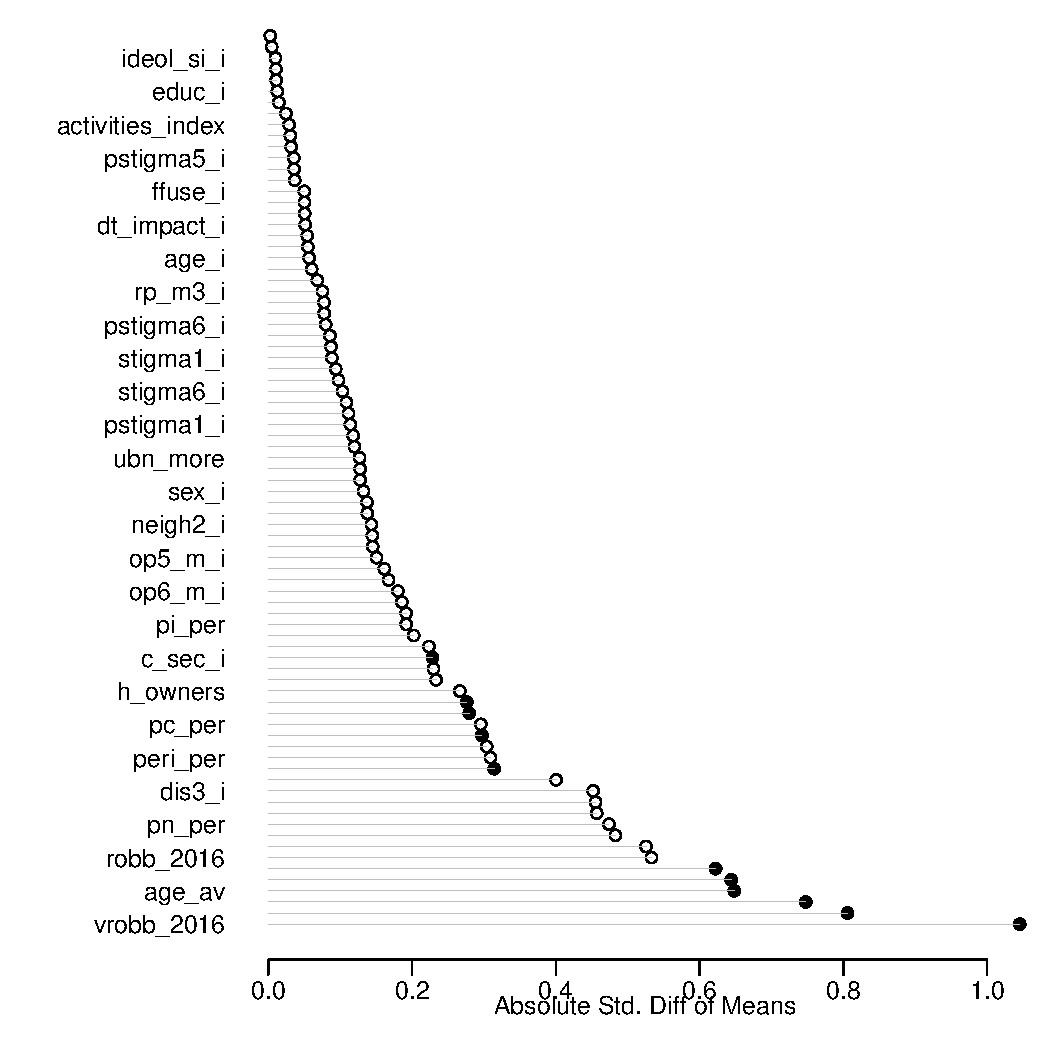
\includegraphics[width=.8\textwidth]{initial_balance_plot.pdf}
\caption{Absolute standardized differences of means between the neighbors of the 16 selling pharmacies and the 42 comparison pharmacies. Although very few differences were larger than 1 sd, approximately 11 differences were inconsistent with random assignment (unadjusted $p \le .05$ (colored with black dots). The omnibus balance test across all 81 covariate relationships produces a $p=.07$ \citep{hansen2008cbs}.We apologize for the cryptic labeling in this draft!} \label{fig:initbal}
\end{figure}

\subsection{Designing a better baseline comparison}

If we had managed to convince the government to issue the registrations by lottery and if a large pool of pharmacies had entered the lottery, we would be able to say that the pharmacies and nearby neighborhoods selected by lottery to sell marijuana would be no different from the pharmacies and associated neighborhoods losing the lottery. This would also be the case if the lottery occurred in groups of places --- say, the right to sell were randomly assigned among pharmacies in Montevideo and also among pharmacies outside of Montevideo. This kind of design would yield a block-randomized experiment. If Montevideo/Interior were the only observed covariate that might confound our comparison, we could directly compare pharmacies to each other within area, and we could compare that stratified design to a hypothetical block-randomized experiment in order to assess the comparison (just as we did above when we compared the simple selling-vs-not selling comparison to a simple randomized experiment with 16 treated and 42 control groups and 81 background covariates). This is what we do below. We use an optimization strategy to produce a series of strata that collectively, across 81 observed covariates, compares favorably to a hypothetical block-randomized experiment. Of course, we do not claim that a stratified design substitutes for an experiment --- we can only speak to differences on 81 covariates, not on all possible observed and unobserved as we could if we had an actually randomized experiment. Later, in \S~\ref{sec:sensitivity}, we assess the extent to which we might change our substantive conclusions based on the stratified design due to the influence of unobserved covariates.\footnote{See \citep[Chapter 3]{rosenbaum2010design} for an overview of this method of sensitivity analysis.}


DESCRIBE THE STRATIFICATION IN SUBSTANTIVE TERMS AND ALSO AS COMPARED TO A HYPOTHETICAL BLOCK-RANDOMIZED EXPERIMENT ON 81 COVARIATES.


\section{Outcome Analysis}
Our entire analysis strategy is based on two main comparisons, considering the different status of pharmacies regarding the marijuana sale. The first one is the simplest one. We compare the survey responses of neighbors of all pharmacies registered to sell marijuana in the time period of our study (n=373), which includes ``wholetime'', ``dropouts'' and ``newcomers'', with the survey responses of neighbors of pharmacies in the control group (n=885), conditioning on matched set.\footnote{We name this group as ``Active''. It takes into account pharmacies that never abandoned the sale, the ones that dropped out at some point and the ones that joined after baseline.}

A second comparison is between neighbors of pharmacies that sold marijuana at the beginning of the implementation of the policy (n=333), which includes ``wholetime'' and ``dropouts'', with neighbors of non-selling pharmacies (n=885).

In addition, and in order to provide robustness to the analysis, we compare ``placebo'' pharmacies with actual selling pharmacies. This would help to dismiss a possible self-selection bias brought by specific characteristics of selling pharmacies. As we mentioned, two pharmacies that established contact with the IRCCA to be a part of the dispensary network, never actually started to sell marijuana. We consider this two cases as placebos. In this case, placebos neighbors (n=40) would be compared with neighbors of all kind of selling pharmacies (n=373). The expectation is to find an effect if the effect is about selling. Another version of this match would be a comparison between placebo and neighbors of non-selling pharmacies (n=885), with the expectation of no effect if the effect is about selling.

Finally, we will compare pharmacies depending on the time they have been selling: neighbors of ``wholetime'' pharmacies (n=207) that were exposed to the selling during the entire period of analysis versus neighbors of pharmacies that, either because they dropped out or because they join later, did not sale the whole time of this study (n=166), ``dropouts'' and ``newcomers'' together that we named them ``part-time.'' We expect larger effects on the 10 selling that have been selling the whole time.

\subsection{Preliminary Results before Stratification and Covariance Adjustment}
\hl{In this version of the paper we show the results of the second proposed comparison between neighbors of pharmacies that sold marijuana at the beginning of the implementation of the policy, which includes ``wholetime'' and ``dropouts'', with neighbors of non-selling pharmacies. Below we present the results of the ATE model for the eight outcomes related to crime victimization, public security, and perceived law impacts.

Having a marijuana selling pharmacy in the neighborhood does not have an impact on crime victimization, as it was expected. Neither there is an effect on country or neighborhood public insecurity perceptions. Neighborhood pharmacies selling marijuana do not change the perceived impact of the law on public security, and they do not alter citizens insertion in the neighborhood. In that sense, after the implementation of marijuana selling at pharmacies, neighbors of those dispensaries behave in the same way that other Uruguayans do in their daily routines and activities (see Table ~\ref{tab:regtab}). Despite the long lines of people outside pharmacies waiting to buy marijuana that became part of the urban scene since 2017, neighbors of those pharmacies do not feel more insecure or change their daily behaviors in the geographical where their live.

Another outcome that we thought might change due to the existence of a marijuana selling pharmacy is the perceived existence of "bocas" in the neighborhood. The argument is that due to the existence of a legal selling point, "bocas" would dissapear from the neighborhood, probable reallocating in another area. This preliminary analysis show that having a marijuana selling pharmacy close by did not have an impact on the perception of the existence of a "boca" in the neighborhood. At least from the citizens' perception, nothing change on that respect.}

\begin{table}[H]
        \centering
        \footnotesize
        \caption{Differences in differences estimation for outcome variables}
    \label{tab:regtab}
    \begin{tabular}{lccccc}
 & \textbf{N} & \textbf{Coeff.}	&	\textbf{Robust Stand.}	&	\textbf{P value}	&	\textbf{CI 95\% } 		\\	
 &  & 	&	\textbf{Error}	&		&		\\	\hline
Country insecurity  perception	&	1215	&	-.0791165	&	.1030153	&	0.443	&	-.2812253    	.1229923	\\	
Neighborhood insecurity perception	&	1212	&	-.0469921	&	.1071544	&	0.661	&	-.257222    	.1632379	\\
Crime victimization in the last 12 months	&	1217	&	-.041347	&	.0446088	&	0.354	&	-.1288663  	 .0461723	\\	
Perceived impact on drug trafficking &	1057	&	-.2066804 	&	.0953157	&	0.030**	&	 -.3937112  	 -.0196497	\\	
Perceived impact on public security	&	1071	&	-.0337569 	&	.0826017 	&	0.683	&	-.1958376    	.1283237	\\
Reported existence of ``bocas''	&	1215	&	.0054253	&	.0602388	&	 0.928	&	-.112759 	.1236096	\\	
Social disorder index	&	1218	&	-.1596775 	&	.0390902 	&	0.000***	&	-.2363694 	-.0829856	\\	
Citizens insertion in their neighborhood	&	1131	&	.0104118	&	.0271764	&	0.702	&	-.0429104   	 .0637339	\\	\hline
*Significant at 90\%\\
**Significant at 95\%\\
***Significant at 99\% \\~\\
        \end{tabular}
        \end{table}

\hl{We include socio-demographic covarietes (sex, age, education and ideology). Perceptions that the law has an impact on drug trafficking and social disorder index are the only two outcomes on which marijuana selling pharmacies has a significant effect. Uruguayans perceptions about the impact that the law has to fight drug traffic positively changed when they have  a marijuana selling pharmacy in their neighborhood. That might be because they see users buying marijuana at the pharmacy and make the deductive reasoning that those are not buying in the illegal market, and as such, this might undermine drug traffic. 

In the case of social disorder, the evidence goes against the expectation. We hypothesize that having a marijuana selling pharmacy in the neighborhood might generate a higher level of social disorder. That expectation took into account the inconveniences that long lines with users outside the pharmacies could imply for neighbors. But the preliminary evidence indicates that selling pharmacies do not generate more social disorder. At least, this was not registered by interviewers while measuring it in the survey.

Our design makes possible to compare perceptions towards insecurity, either in the country or the neighborhood, through time. The effect of time have worsen both outcomes in the last twelve months. However, this deterioration has nothing to do with marijuana selling pharmacies, and it is consistent with  the national trends.}\footnote{According with data form the LAPOP Project, the percentage of people who declares feeling “very safe” in their neighborhood drops between 2010 and 2014. On the contrary, people that feels “very unsafe” grow in the same period.}

\section{Sensitivity to unobserved confounds} \label{sec:sensitivity}

Our stratified research design successfully adjusted for 81 covariates, but it did not adjust for the many other unobserved differences existing between the selling and not-selling pharmacies.  In this section we ask how severe the unobserved differences would have to be before we would change our substantive interpretation of our results. This kind of sensitivity analysis a formalized what-if exercise because, in fact, we do not know how much unobserved confounding to worry about.

TO DO.

\section{Discussion and Final Remarks}
This paper has a twofold purpose. On one side, it wants to contribute to the literature which tackles the causal effect between crime and marijuana legalization. On the other side, it aims to evaluate the impact of marijuana regulation in Uruguay on insecurity perceptions and crime victimization, and by doing that inform the public policy.

Our evidence shows no impact of marijuana selling at pharmacies on crime victimization. Following the evidence of \cite{dragone2019crime} and the previous research mentioned above, it was plausible to expect that more dispensaries generate lower crime victimization. It is also truth that, considering the small participation of the marijuana trade in the illegal drug market, the effect of marijuana legalization should be moderate. In Caulkins et al.words: ``Where the problem is already modest, the potential changes are also necessarily modest'' (\citet[154]{caulkins2015considering}).

\hl{As we already posed, in the Uruguayan context, where the national crime rates had steadily growth in the last years, we could expect that crime victimization goes upwards both among neighbors of marijuana selling pharmacies and also among others citizens that do not live close by a marijuana dispensary, but it might be a smaller growth among the former. Regarding crime victimization, the preliminary evidence presented in the article does not show that effect.}

\hl{Which are the mechanisms that we believe are behind the link between the legalization of marijuana and crime? More specifically, why would the introduction of legal marijuana dispensaries cause a decrease in crime victimization and the other outcomes associated with public security? The causal mechanisms behind this process might be in line with Dragone's work: moving retail cannabis deals from degraded streets to safe, legal shops most likely played a role as it is posed by Becker and Murphy (2013). Following this argument, if the illegal expenditure points (``bocas'') have less ground to move next to the legal dispensaries, maybe we could be attending to an slipping of the ``bocas'' to neighbors where no legal marijuana dispensaries are located. We found no significant difference on the identification of ``bocas'' made by neighbors before and after the pharmacies started to sell marijuana, and neither between neighbors that live close to a selling pharmacy and those that do not. However, selling pharmacies owners and employees state that ``bocas'' have diminished in the neighborhood. We surveyed all the owners of marijuana selling pharmacies before and after they started to sell marijuana. In 2017, 84,6\% said they knew there was a ``boca'' in the neighborhood, and in 2018 that percentage diminished to 46,1\%. Among owners of non- selling pharmacies, owners did not recognize any change (63,3\% in 2017 and 62,9\% in 2018).}

\hl{In the case of insecurity perceptions, estimations do not show any statistically significant effect between neighbors, meaning that living closed to a selling pharmacies does not modify insecurity perceptions. Perceived impact of the regulation on public security does not present statistically significant differences neither. People not only feel just as insecure in one group or the other, but also they do not visualize the policy as a potential instrument to improve public insecurity, and this does not change when they are directly in contact with the policy. This finding is interesting considering how this policy emerged, the initial frame that the government used to present the bill, and its specific aims regarding public security. Apparently the link between drugs regulation and crime is not so obvious for treated neighbors either.}

\hl{On the contrary, people who live near a selling pharmacy believe that the regulation is improving the fight against drug trafficking, in contrast with people who does not live near one. Although we do not have much information on the casual mechanisms behind this perception, it might be that regular contact with consumers persuade people to consider that the sale at pharmacies it is actually a way of reducing illegal drug markets, not forcing ordinary people to be in contact with dealers or in the illegal expenditures points. In other words, being in straight contact with the policy improves the perceived impact against the illegal market. An unexpected result is that marijuana selling pharmacies reduce social disorder in the neighborhood. This preliminary finding goes against our expectation and needs further research.}

\hl{As it was stated at the beginning, the purpose of this paper is to make a contribution to the public policy discussion on whether marijuana legalization produce social goods or not. Uruguay was the first country to fully regulate the marijuana market, Canada the second in 2018, and it is probable that more countries would follow the same path. As a result, it is extremely relevant to understand the effects of those legalizations on different social, economic and political outcomes. In particular it looks at a series of outcomes that were key in the Uruguayan legalization policy process: crime and public insecurity perception. The data analysis presented in this version is a first cut. We need to perform a computational matching to analyze the results by clusters of similar pharmacies, in order to compare selling and non-selling pharmacies in a way that comes close to a hypothetical block-randomized experiment, despite we know that there might be always unobserved variables that might have an effect on our outcomes of interest.}


\printbibliography[title={8 References}]

\newpage
\appendix % is redefined by hyperref and a mess, do the appendix stuff by hand instead
% problems with pdf bookmarks and appendix caused by resetting section counter.
% solution here: http://www.latex-community.org/forum/viewtopic.php?f=45&t=4950
%\begin{singlespacing}
\newcounter{mycounter}
\setcounter{mycounter}{0}
\let\osection\section
\renewcommand{\section}{\stepcounter{mycounter}\osection}
\renewcommand\thesection{Appendix \Alph{mycounter}}

\section{Pharmacies Description}
\begin{samepage}
\begin{table}
    \begin{small}
    \centering
    \caption{Pharmacies´Infrastructure and Representatives Perceptions About Insecurity, Marijuana Regulation, ts Impacts and Use}
    \addtolength{\tabcolsep}{-3pt}
    \label{tab:pharmaciesperceptions}
    \begin{tabular}{lcccc}
	&	Non-selling	&		&	Selling	&		\\	
	&	N	&	\%	&	N	&	\%	\\	\hline
\textbf{Pharmacies' general characteristics	}&		&		&		&		\\	\hline
5 stores or less	&	35	&	83,3	&	17	&	100	\\	
Average number of employees	&	42	&	5,1*	&	17	&	5,4*	\\	
Average years of functioning 	&	42	&	40.1*	&	17	&	36.8*	\\	
Family business	&	27	&	65,8\%	&	13	&	81,2\%	\\	\hline
\textbf{Pharmacies' infrastructure}	&		&		&		&		\\	\hline
Alarm with response	&	35	&	83,3\%	&	9	&	56,2\%	\\	
Security guard during the day &	&	5	&	11,9\%	&	2	&	12,5\%	\\	
Security cameras 	&	26	&	63,4\%	&	14	&	87,5\%	\\	
Security guard during the night	&	3	&	7,14\%	&	3	&	18,7\%	\\	
Bars and intercom at the door	&	3	&	7,2\%	&	2	&	12,5\%	\\	
No security measures at the door	&	21	&	51,2\%	&	9	&	56,2\%	\\	\hline
\textbf{Insecurity perceptions and crime}	&		&		&		&		\\	\hline
Crime victimization 	&	15	&	25,7\%	&	3	&	17,65	\\	
Perceptions of "Somewhat unsafe" and "Very unsafe"	&	15	&	51,7\%	&	10	&	62,5\%	\\	
Reported existence of "bocas"	&	19	&	63,3\%	&	11	&	84,6\%	\\	
Trust in people of the neighborhood	&		&		&		&		\\	
("Very trustworthy" and "Somewhat trustworthy")	&	36	&	92,3	&	17	&	100	\\	\hline
\textbf{Opinions about the policy}	&		&		&		&		\\	\hline
Agreement with marijuana regulation 	&		&		&		&		\\	
("Strongly agree" and "Agree")	&	16	&	39\%	&	13	&	81\% 	\\	
Agreement with sale at pharmacies	&		&		&		&		\\	
 ("Strongly agree" and "Agree")	&	6	&	14,6\%	&	14	&	82\%	\\	
Positive impact on public health 	&	2	&	5,9\%	&	4	&	23,5\%	\\	
Positive impact on public security 	&	2	&	5,7\%	&	2	&	12,5\%	\\	
Positive impact on fight against drug-trafficking	&	12	&	32,4\%	&	5	&	33,3\%	\\	
Positive impact on individual liberties	&	9	&	23,1\%	&	7	&	43,7\%	\\	\hline
\textbf{Opinions about the substance and its users}	&		&		&		&		\\	\hline
Agreement with "marijuana users	&		&		&		&		\\	
are a threat to society"**	&	6	&	14,3\%	&	0	&	0	\\	
Agreement with "marijuana is a gateway drug"**	&	15	&	35,7\%	&	4	&	22,7\%	\\	
Agreement with "marijuana use 	&		&		&		&		\\	
is detrimental to health"**	&	13	&	31\%	&	4	&	25\%	\\	\hline
\end{tabular}
\end{small}
\newline
\tiny{*Mean number \\
**Percentages showed are more radical positions (values 6 and 7) on a scale from 1 to 7, 1 being "Strongly disagree" and 7 being "Strongly agree".}
\end{table}
\end{samepage}


\newpage
\newgeometry{margin=1cm}
\begin{landscape}
  \tiny
\begin{longtable}[htbp]{@{}p{1.2cm}p{1cm}p{1.5cm}p{1cm}p{1cm}p{1cm}p{1cm}p{1cm}p{1cm}p{1cm}p{1cm}p{1.2cm}p{1cm}p{1cm}@{}}
%\centering
  \caption{Indicators for Selected  Pharmacies} \\
  \label{tab:phlongtable}
\toprule

Neighborhood / Locality	&	Pharmacy`s name	&	Administrative Region (departamento)	&	Treatment	&	Number of assaults per Neighborhood / Locality	&	Number of assaults per administrative region	&	Number of robberies per Neighborhood / Locality	&	Number of robberies per administrative region	&	Number of homicides per administrative region	&	Total population of the admnistrative region	&	Total population of the Neighborhood / Locality	&	Neighborhood / Locality`s population density	&	Average income of the Neighborhood / Locality	&	Average age of the Neighborhood / Locality	\tabularnewline
\midrule
\endhead

Malvin Norte	&	Pitagoras	&	Montevideo	&	Yes	&	871	&	11409	&	184	&	31.137	&	113	&	1.305.082	&	19.916	&	11.620	&	19.302	&	39	\tabularnewline
Cordon	&	Galena	&	Montevideo	&	No	&	1469	&	11409	&	222	&	31.137	&	113	&	1.305.082	&	42.456	&	18.629	&	29.580	&	39	\tabularnewline
Aguada	&	Roosevelt	&	Montevideo	&	No	&	514	&	11409	&	514	&	31.137	&	113	&	1.305.082	&	18.557	&	8.982	&	25.982	&	40	\tabularnewline
Belvedere	&	Belvedere	&	Montevideo	&	No	&	480	&	11409	&	480	&	31.137	&	113	&	1.305.082	&	21.970	&	6.861	&	18.376	&	41	\tabularnewline
Paso Molino	&	Mastil	&	Montevideo	&	No	&	0	&	11409	&	0	&	31.137	&	113	&	1.305.082	&	21.970	&	6.861	&	18.376	&	40	\tabularnewline
Pocitos	&	Brito del Pino	&	Montevideo	&	No	&	1221	&	11409	&	171	&	31.137	&	113	&	1.305.082	&	67.992	&	21.660	&	42.403	&	44	\tabularnewline
Sayago	&	Farmacia Ariel	&	Montevideo	&	No	&	626	&	11409	&	189	&	31.137	&	113	&	1.305.082	&	14.692	&	5.625	&	21.465	&	38	\tabularnewline
Cordon	&	La caja	&	Montevideo	&	No	&	1469	&	11409	&	222	&	31.137	&	113	&	1.305.082	&	42.456	&	18.629	&	29.580	&	38	\tabularnewline
Curva de Maroñas	&	Lulisan	&	Montevideo	&	No	&	0	&	11409	&	239	&	31.137	&	113	&	1.305.082	&	20.812	&	7.133	&	15.591	&	41	\tabularnewline
Parque Rodo	&	Farmashop 50	&	Montevideo	&	No	&	429	&	11409	&	0	&	31.137	&	113	&	1.305.082	&	12.944	&	16.898	&	33.781	&	41	\tabularnewline
Ciudad Vieja	&	Cielmar	&	Montevideo	&	No	&	593	&	11409	&	0	&	31.137	&	113	&	1.305.082	&	12.555	&	5.947	&	23.112	&	41	\tabularnewline
Union	&	Milena	&	Montevideo	&	No	&	1582	&	11409	&	299	&	31.137	&	113	&	1.305.082	&	39.880	&	9.975	&	21.562	&	43	\tabularnewline
Buceo	&	Farmashop 58	&	Montevideo	&	No	&	1155	&	11409	&	251	&	31.137	&	113	&	1.305.082	&	36.998	&	8.905	&	27.440	&	43	\tabularnewline
Brazo oriental	&	Farmacia Goñi Central	&	Montevideo	&	No	&	456	&	11409	&	0	&	31.137	&	113	&	1.305.082	&	16.812	&	8.976	&	21.519	&	43	\tabularnewline
Sayago	&	Sangar	&	Montevideo	&	No	&	626	&	11409	&	189	&	31.137	&	113	&	1.305.082	&	14.692	&	5.625	&	21.465	&	43	\tabularnewline
La Blanqueada	&	Guarani	&	Montevideo	&	No	&	0	&	11409	&	0	&	31.137	&	113	&	1.305.082	&	9.600	&	12.245	&	31.489	&	43	\tabularnewline
Parque Batlle	&	FARMASHOP 52	&	Montevideo	&	No	&	1049	&	11409	&	185	&	31.137	&	113	&	1.305.082	&	31.153	&	9.231	&	36.782	&	40	\tabularnewline
Cordon	&	Pigalle	&	Montevideo	&	No	&	1469	&	11409	&	222	&	31.137	&	113	&	1.305.082	&	42.456	&	18.629	&	29.580	&	43	\tabularnewline
Malvin	&	El tunel	&	Montevideo	&	No	&	871	&	11409	&	217	&	31.137	&	113	&	1.305.082	&	28.102	&	8.027	&	37.732	&	40	\tabularnewline
Malvin	&	San Roque	&	Montevideo	&	No	&	871	&	11409	&	217	&	31.137	&	113	&	1.305.082	&	28.102	&	8.027	&	37.732	&	40	\tabularnewline
Centro	&	Antartida	&	Montevideo	&	Yes	&	1120	&	11409	&	173	&	31.137	&	113	&	1.305.082	&	22.120	&	17.055	&	34.049	&	44	\tabularnewline
Pocitos	&	CACERES	&	Montevideo	&	Yes	&	1221	&	11409	&	171	&	31.137	&	113	&	1.305.082	&	67.992	&	21.660	&	42.403	&	44	\tabularnewline
Ciudad vieja	&	Tapie	&	Montevideo	&	Yes	&	593	&	11409	&	0	&	31.137	&	113	&	1.305.082	&	12.555	&	5.947	&	23.112	&	43	\tabularnewline
Aguada	&	Sildia	&	Montevideo	&	No	&	514	&	11409	&	514	&	31.137	&	113	&	1.305.082	&	18.557	&	8.982	&	25.982	&	43	\tabularnewline
La Blanqueada	&	Quintela	&	Montevideo	&	No	&	0	&	11409	&	0	&	31.137	&	113	&	1.305.082	&	9.600	&	12.245	&	31.489	&	41	\tabularnewline
Ciudad de Artigas	&	Saga	&	Artigas	&	Yes	&	14	&	25	&	386	&	1.647	&	0	&	73.377	&	40.658	&	2.740	&	11.733	&	36	\tabularnewline
Bella Unión	&	Santa Cecilia Centro	&	Artigas	&	No	&	7	&	25	&	2	&	1.647	&	0	&	73.377	&	40.658	&	2.740	&	11.733	&	36	\tabularnewline
Ciudad de Artigas	&	Horandre	&	Artigas	&	No	&	14	&	25	&	386	&	1.647	&	0	&	73.377	&	40.658	&	2.740	&	11.733	&	36	\tabularnewline
Las Toscas	&	Las toscas	&	Canelones	&	Yes	&	38	&	2165	&	1160	&	11.490	&	26	&	520.173	&	3.146	&	1.022	&		&		\tabularnewline
Ciudad de Canelones	&	miguel	&	Canelones	&	Yes	&	57	&	2165	&	706	&	11.490	&	26	&	520.173	&	19.865	&	1.582	&	19.130	&	40	\tabularnewline
Parque del Plata	&	bologna	&	Canelones	&	No	&	38	&	2165	&	1160	&	11.490	&	26	&	520.173	&	7.896	&	945	&		&		\tabularnewline
Ciudad de Canelones	&	Pirujas	&	Canelones	&	No	&	57	&	2165	&	706	&	11.490	&	26	&	520.173	&	19.865	&	1.582	&	19.130	&	40	\tabularnewline
Pando	&	Farmacia central	&	Canelones	&	No	&	169	&	2165	&	1045	&	11.490	&	26	&	520.173	&	25.947	&	2.471	&		&		\tabularnewline
Carmelo	&	Carmelo	&	Colonia	&	Yes	&	2	&	20	&	434	&	1.971	&	3	&	123.203	&	18.041	&	1.512	&	15.117	&	38	\tabularnewline
Nueva Palmira	&	Arrieta	&	Colonia	&	No	&	4	&	20	&	100	&	1.971	&	3	&	123.203	&	9.857	&	528	&	15.947	&	38	\tabularnewline
Carmelo	&	Ferrer	&	Colonia	&	No	&	2	&	20	&	434	&	1.971	&	3	&	123.203	&	18.041	&	1.512	&	15.117	&	38	\tabularnewline
Trinidad	&	Nueva Brun	&	Flores	&	Yes	&	15	&	7	&	644	&	396	&	0	&	25.050	&	21.429	&	3.221	&	15.694	&	40	\tabularnewline
Trinidad	&	Osta	&	Flores	&	No	&	15	&	7	&	644	&	396	&	0	&	25.050	&	21.429	&	3.221	&	15.694	&	40	\tabularnewline
Ismael Cortinas	&	Vidal	&	Flores	&	No	&	0	&	7	&	12	&	396	&	0	&	25.050	&	918	&	963	&		&		\tabularnewline
Minas	&	Gortari	&	Lavalleja	&	Yes	&	27	&	17	&	647	&	1.009	&	5	&	58.815	&	38.446	&	2.135	&	15.879	&	37	\tabularnewline
Minas	&	Idamar	&	Lavalleja	&	No	&	27	&	17	&	647	&	1.009	&	5	&	58.815	&	38.446	&	2.135	&	15.879	&	37	\tabularnewline
Minas	&	Williman 2	&	Lavalleja	&	No	&	27	&	17	&	647	&	1.009	&	5	&	58.815	&	38.446	&	2.135	&	15.879	&	37	\tabularnewline
Las Flores	&	La Cabina	&	Maldonado	&	Yes	&	0	&	212	&	102	&	6.238	&	12	&	164.298	&	241	&	229	&		&		\tabularnewline
San Carlos	&	Alvariza	&	Maldonado	&	No	&	43	&	212	&	755	&	6.238	&	12	&	164.298	&	27.471	&	3.656	&	16.948	&	38	\tabularnewline
Maldonado	&	Maldonado	&	Maldonado	&	No	&	31	&	212	&	1106	&	6.238	&	12	&	164.298	&	62.590	&	4.916	&	16.127	&	36	\tabularnewline
Ciudad de Paysandú	&	Medicci	&	Paysandú	&	Yes	&	38	&	74	&	834	&	2.635	&	4	&	113.107	&	76.412	&	3.539	&	15.082	&	38	\tabularnewline
Villa Quebracho	&	Guaviyu	&	Paysandú	&	No	&	0	&	74	&	33	&	2.635	&	4	&	113.107	&	2.853	&	2.202	&	.	&	.	\tabularnewline
Termas de Guaviyú	&	Termal guaviyu	&	Paysandú	&	Yes	&	0	&	74	&	19	&	2.635	&	4	&	113.107	&	38	&	44	&	.	&	.	\tabularnewline
Guichón	&	Lombardi/Guichón	&	Paysandú	&	No	&	1	&	74	&	19	&	2.635	&	4	&	113.107	&	5.039	&	1.577	&	10.181	&	37	\tabularnewline
Ciudad de Paysandú	&	San Roque	&	Paysandú	&	No	&	29	&	74	&	534	&	2.635	&	4	&	113.107	&	76.412	&	3.539	&	15.082	&	38	\tabularnewline
Ciudad de Paysandú	&	Dorotte II	&	Paysandú	&	No	&	29	&	74	&	534	&	2.635	&	4	&	113.107	&	76.412	&	3.539	&	15.082	&	38	\tabularnewline
Dayman	&	Albisu Termal	&	Salto	&	Yes	&	17	&	122	&	1187	&	2.978	&	7	&	124.861	&	356	&	209	&		&		\tabularnewline
Ciudad de Salto	&	Farmacia Pasteur	&	Salto	&	No	&	16	&	122	&	804	&	2.978	&	7	&	124.861	&	104.011	&	2.812	&	16.209	&	38	\tabularnewline
Ciudad de Salto	&	Nueva Republica	&	Salto	&	No	&	16	&	122	&	804	&	2.978	&	7	&	124.861	&	104.011	&	2.812	&	16.209	&	38	\tabularnewline
Libertad	&	Bedegain	&	San José	&	Yes	&	10	&	143	&	440	&	1.815	&	2	&	108.304	&	10.167	&	1.764	&	15.757	&	37	\tabularnewline
Ciudad del Plata	&	Del 26	&	San José	&	No	&	109	&	143	&	507	&	1.815	&	2	&	108.304	&	31.146	&	1.200	&	21.655	&	37	\tabularnewline
San José de Mayo	&	Bellini	&	San José	&	No	&	20	&	143	&	646	&	1.815	&	2	&	108.304	&	36.743	&	2.641	&	18.934	&	40	\tabularnewline
Paso de los Toros	&	Bengoechea	&	Tacurembó	&	Yes	&	1	&	16	&	93	&	907	&	6	&	90.051	&	12.985	&	1.341	&	12.768	&	36	\tabularnewline
Paso de los Toros	&	Demilton	&	Tacurembó	&	No	&	1	&	16	&	93	&	907	&	6	&	90.051	&	12.985	&	1.341	&	12.768	&	36	\tabularnewline
Tacuarembó	&	Dini	&	Tacurembó	&	No	&	19	&	15	&	600	&	907	&	6	&	90.051	&	54.757	&	1.721	&	13.940	&	37	\tabularnewline
Pocitos	&	Camaño	&	Montevideo	&	Yes	&	1221	&	11409	&	171	&	31.137	&	113	&	1.305.082	&	67.992	&	21.660	&	42.403	&	44	\tabularnewline
Brazo oriental	&	Silleda	&	Montevideo	&	Yes	&	456	&	11409	&	0	&	31.137	&	113	&	1.305.082	&	16.812	&	8.976	&	21.519	&	43	\tabularnewline
Flor de Maroñas	&	Constitución Sur	&	Montevideo	&	Yes	&	0	&	11409	&	239	&	31.137	&	113	&	1.305.082	&	20.812	&	7.133	&	15.591	&	42	\tabularnewline
Punta Carretas	&	Lilen	&	Montevideo	&	Yes	&	617	&	11409	&	170	&	31.137	&	113	&	1.305.082	&	24.181	&	8.858	&	46.759	&	43	\tabularnewline

\bottomrule
\end{longtable}

Source: Own elaboration. *Population data from National Census (2011). **Income and age data from National Household Survey (2017). *** Criminality data per administrative regions from Ministry of Interior (1st. semester 2018) ****Criminality data per neighborhoods in Montevideo from Ministry of Interior (1st. semester 2018).*****Criminality data per localities in the rest of the country from Ministry of Interior (2016).
\end{landscape}
\restoregeometry

\newgeometry{margin=1cm}
\begin{landscape}
\section{Outcome Variable Description}
\begin{tiny}
\begin{tabular}{lllcc}
\textbf{Variable }	&	\textbf{Survey question} 	&	\textbf{Scale}	&	\textbf{Min.}	&	\textbf{Max.}		\\	\hline
Country insecurity  perception	&	In general, in your country, do you feel very safe	&	1. Very unsafe 	&	1	&	4	\\
	&	somewhat unsafe or very unsafe?	&	2. Somewhat unsafe 	&		&		\\
	&		&	3. Somewhat safe 	&		&		\\
	&		&	4. Very safe 	&		&		\\\hline
Neighborhood 	&	And in the neighborhood where you live, 	&	1. Very unsafe 	&	1	&	4	\\
insecurity perception	&	do you feel very safe, somewhat safe,	&	2. Somewhat unsafe 	&		&		\\
	&	somewhat unsafe or very unsafe?	&	3. Somewhat safe 	&		&		\\
	&		&	4. Very safe 	&		&		\\\hline
Crime victimization in the last 	&	Now, changing the subject, have you been a victim of 	&	0. Yes	&	0	&	1	\\
12 months	&	any type of crime in the past 12 months? That is, have	&	1. No 	&		&		\\
	&	you been a victim of robbery, burglary, assault, fraud,	&		&		&		\\
	&	blackmail, extortion, violent threats or any other type	&		&		&		\\
	&	of crime in the past 12 months?	&		&		&		\\\hline
Perceived impact on public security	&	Now regarding to public safaty, because of this law,	&	1.  Worst (is already worst)	&	1	&	3	\\
	&	 do you think the country will be better, will 	&	2. Same	&		&		\\
	&	remain the same or will be worst?	&	3. Better (is already better)	&		&		\\\hline
Perceived impact on drug trafficking	&	Now regarding to drug trafficking, because of this law,	&	1.  Worst (is already worst)	&	1	&	3	\\
	&	 do you think the country will be better, will 	&	2. Same	&		&		\\
	&	remain the same or will be worst?	&	3. Better (is already better)	&		&		\\\hline
Reported existence of bocas	&	Based on what you know or hear, there is a any boca	&	0. Yes	&	0	&	1	\\
	&	in this area?	&	1. No 	&		&		\\\hline
Social disorder index	&	Built with the folllowing questions:	&	1. Very much	&	1	&	4	\\
	&		&	2. Somewhat	&		&		\\
	&		&	3. Llittle	&		&		\\
	&		&	4. Not at all	&		&		\\
Presence of young people or children 	&	Observational	&	1. Very much	&	1	&	4	\\
in the streets without doing	&		&	2. Somewhat	&		&		\\
 anything, who are wandering	&		&	3. Llittle	&		&		\\
	&		&	4. Not at all	&		&		\\
Presence of   people drunk or 	&	Observational	&	1. Very much	&	1	&	4	\\
stoned in the streets	&		&	2. Somewhat	&		&		\\
	&		&	3. Llittle	&		&		\\
	&		&	4. Not at all	&		&		\\
Presence of people discussing in 	&	Observational	&	1. Very much	&	1	&	4	\\
aggressive or violent (speaking in 	&		&	2. Somewhat	&		&		\\
a tone of voice very high, 	&		&	3. Llittle	&		&		\\
with anger)	&		&	4. Not at all	&		&		\\\hline
Citizens insertion in 	&	Built with the folllowing questions:	&		&		&		\\
neighborhood*	&		&	-	&	0	&	1	\\
Talk with your neighbors	&	Finally, thinking about the activities you do in 	&	1. Never	&		&		\\
	&	this neighborhood, please tell me how many times you:	&	2. Once or twice a year	&	1	&	4	\\
	&	talk with your neighbors	&	3. Once or twice a month	&		&		\\
	&		&	4. Once a week	&		&		\\
Organize meetings with the 	&	Finally, thinking about the activities you do in 	&	1. Never	&		&		\\
neighbors to improve 	&	this neighborhood, please tell me how many times you:	&	2. Once or twice a year	&	1	&	4	\\
the neighborhood	&	organize meetings with the 	&	3. Once or twice a month	&		&		\\
	&	neighbors to improve the neighborhood	&	4. Once a week	&		&		\\
Use educational services 	&	Finally, thinking about the activities you do in 	&	1. Never	&	1	&	4	\\
(kindergarten, school, high school)	&	this neighborhood, please tell me how many times you:	&	2. Once or twice a year	&		&		\\
 in the neighborhood	&	use educational services (kindergarten, school, 	&	3. Once or twice a month	&		&		\\
	&	high school) in the neighborhood	&	4. Once a week	&		&		\\
Use health services 	&	Finally, thinking about the activities you do in 	&	1. Never	&		&		\\
(doctor, hospital) of the	&	this neighborhood, please tell me how many times you:	&	2. Once or twice a year	&	1	&	4	\\
neighborhood	&	use health services (doctor, hospital) of the	&	3. Once or twice a month	&		&		\\
	&	neighborhood	&	4. Once a week	&		&		\\
Buy at the shops in the 	&	Finally, thinking about the activities you do in 	&	1. Never	&		&		\\
neighborhood	&	this neighborhood, please tell me how many times you:	&	2. Once or twice a year	&	1	&	4	\\
	&	buy at the shops in the neighborhood	&	3. Once or twice a month	&		&		\\
	&		&	4. Once a week	&		&		\\
Do recreational activities 	&	Finally, thinking about the activities you do in 	&	1. Never	&		&		\\
in the neighborhood	&	this neighborhood, please tell me how many times you:	&	2. Once or twice a year	&	1	&	4	\\
	&	do recreational activities in the neighborhood	&	3. Once or twice a week	&		&		\\
	&		&	4. Once a week	&		&		\\\hline
*Standarized
\end{tabular}
\end{tiny}

\end{landscape}
\restoregeometry


\newpage The social disorder index was built using three variables: presence of young people loitering, presence of drunk or stoned people in the streets, and presence of people arguing with each other. Each of these variables have the following values: 1 (Very much), 2 (Somewhat), 3 (Little), and 4 (Not at all). In order to construct the index we assume intermediate substitutability among variables and assign the mean value \citep{goertz2006social}.

Citizens' Insertion on their Neighborhood is an index constructed with eight variables grouped in four dimensions. The dimensions are: use of services (education and health) in the neighborhood, contact among neighbors (chat and/or meet for collective action activities), perform recreational activities in the neighborhood, and shopping in the neighborhood. We assume intermediate substitutability among dimensions and assign the mean value. The use of services dimension has two indicators: use of educational services (kindergarten, school,high school) in the neighborhood and use of health services (doctor, hospital) in the neighborhood. We assume total substitutability among the two indicators and assign the maximum value  \citep{goertz2006social}.Contact among neighbors dimension also has two indicators: talk with your neighbors and meets/ organizes with the neighbors for any improvement activity for the neighborhood. We also assume total substitutability among the two indicators and assign the maximum value. Perform recreational activities in the neighborhood is measured by the question: do you perform any recreational activities in the neighborhood? Finally, shopping in the neighborhood is measured by the question: do you purchase in warehouses or stores in the neighborhood? Each indicator is measured using the same scale:1 (Never), 2 (Once or twice a year), 3 (Once or twice a month), and 4 (Once a week).  Citizens' insertion is an index standardized, values go from 0 to 1.

\section{Details of the search for stratification}
Here we will describe in more detail how we used a full optimal matching algorithm \citep{hansen:2004} to find a stratified comparison between selling and non-selling pharmacies that met the standard of comparing favorably with a hypothetical block-randomized experiment.

\section{Threats to Inference: Attrition and Spillovers}
One problem for this design could be sample attrition. It is possible that some people moved, leaving either the treatment or the control group. In general, moving is not a frequent behavior in Uruguay. Although we do not know for sure how many respondents from the baseline survey moved before the second round, we do know that only 4.33 percent (n=30) of those interviewed in the second round moved after we run the baseline.

We minimize spillover between pharmacies by ensuring that the comparison pharmacies were at least 6 blocks away from the selling pharmacies.
\end{document}
